% NOTE:  I suggestion we rename this subsection.  Whenever optimization is 
%   used, the term smoothing is no longer used, as smoothing can lead
%   to a decrease in the metric being measured.  With mesh quality, the 
%   appropriate term is mesh quality improvement.  I would have used the 
%   term mesh representation deficit improvement here.  However, since
%   this is a subsection and all subsection titles should be parallel,
%   that doesn't quite work either.  Can you think of a better title?

\subsection{Nodal Smoothing}
In this paper, the focus is on using nodal smoothing in 
order to locally minimize the representation deficit in the surface mesh.  
It should be noted that, although a locally optimal mesh topology could 
also be obtained, computing such a topology would involve the solution of 
a discrete optimization problem (via integer programming) which would 
specify the relevant sequence of edge flips.  The discrete 
and continuous optimization problems could then be solved in an iterative, 
interleaving fashion.  However, such an approach would require significant 
additional computational expense.

For a node, $N_i$, the representation deficit is defined only by
comparing it to the node when located at another point in space. Here
the comparison is bound by limiting the range of comparison within the
edge-hull topologically adjacent to $N_i$. Formally, let $N_i$ be a node
in $D$ that is shared topologically by $n$ triangles, where $n$ is the
face-valence of $N_i$. The optimization for finding the optimal position
for $N_i$ is defined as:

\begin{eqnarray*}
\begin{array}{rcl}
\underset{N_O}{\text{minimize}} \ O(N) & = &
-\sum{_{j=1}^{n_t-1}A\left(T_j\right)} \\
\text{subject to} \ N_{T_1} & > & 0 \\
N_{T_2} & > & 0 \\ 
N_{T_3} & > & 0 \\
& \vdots & \\
N_{T_{n-1}} & > & 0 \\ 
N_{T_n} & > & 0.
\end{array}
\end{eqnarray*}

\begin{figure}[h!]
  \center{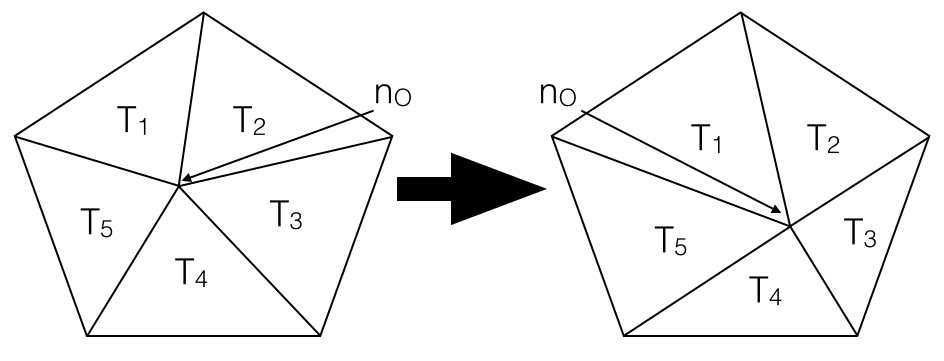
\includegraphics[height=1.4in]
    {Figures/NodalSmoothing.jpg}}
  \caption{Nodal Smoothing}
\end{figure}

[NEED TO DISCUSS HESSIAN/METRIC BASED MESH ADAPTION IN THE NODAL
SMOOTHING SECTION OF THE PAPER. THERE IS NO GLOBAL, STATIC FUNCTION
AGAINST WHICH THE INTERPOLATION ERROR CAN BE MINIMIZED. THAT IS,
WHENEVER THE MESH MOVES, THE INTERPOLATION ERROR FIELD CHANGES.]
